\subsection{Trajectory Extraction}
\label{sec:trajectory_extraction}

Our system extracts trajectories from location-based social media data.
Users first select a geographical boundary and a target time window of interest.
% or a real time mode.
The users additionally select one or more past time windows representing normal situations to compare against the target time frame.
The trajectory extraction module then requests two sets of Tweets from the database for the two selected time windows.
%Two sets of the tweets generated within the each time windows.
The module generates two sets of trajectories: target and normal trajectories using geo-location information of chronologically ordered Tweets for each person.

\begin{figure}[tbh]
	\centering
	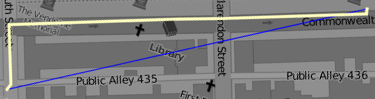
\includegraphics[width=0.8\linewidth]{route_v2}
	\caption{Supplementing a sparse trajectory (Blue) using route direction information (Yellow). }
	\label{fig:route}
	%\vspace{-0.4cm}
\end{figure}

%The extracted raw trajectories, however, do not have enough fine-grained spatial positions.
The generated trajectories, however, are usually sparse and incomplete.
%compared to ones generated by GPS devices (the interval is a couple of seconds between each point).
For example, as shown in Figure~\ref{fig:route}, the sparse trajectory (a blue line) does not represent a realistic movement.
In order to reduce the spatial sparseness of the raw trajectories, 
we fill the trajectories with supplementary points between two points for each pair of the trajectories, which are calculated by shortest-path-based route directions (a yellow poly line in Figure~\ref{fig:route}).
%We compensate the sparse positions in the trajectories using route information between each position.
%In this work, we use geo-location information extracted from tweets to build trajectories of each user.
%However, the temporal intervals between each posting have a high degree of variation\textemdash a couple of from minutes to hours.
%Therefore, it is hard to find realistic movements using the high sparse trajectories.
%The abstraction level of the trajectories is too high to obtain actuality.
%We need appropriate fine-grained spatial positions between the recorded positions.
In this work, we use the Bing Maps API to obtain route information.
We can choose one of the following travel modes: walking, driving, or public transportation mode depending on the location and the situation.
For example, we select the walking mode for the Boston Marathon case because many traffic routes along the marathon course were closed on the race day.
%The Google Maps API also provide a route calculation service, but for the public license users, the number of requests is limited.

%\begin{itemize}
%\item Finding references showing how much the shortest route is similar to the real movement
%\end{itemize}